% 最小二乘法曲线拟合

\pentry{最小二乘法\upref{LstSqr}, Nelder-Mead 算法\upref{NelMea}}
我们在 “最小二乘法\upref{LstSqr}” 中见到的三个例子中, 方差函数都是待定系数的线性组合, 这种情况下我们令偏导为零后得到的是线性方程组, 便于求解%(见 Matlab 或 Mathematica)链接未完成. 
. 然而当方差不是待定系数的线性组合时, 得到的方程组往往非常复杂, 这时就需要借助数值计算. 相比用数值计算解 $N$ 元的非线性方程组, 更简单的方法是直接用数值方法寻找方差函数的极小值(如Nelder-Mead 算法) . 实践证明, 大多数情况下极小值点仅有一个, 那就是最小值点.

为了验证结果的正确性, 我们先来用数值方法拟合 $A\cos (x + \varphi_0) + C$, 并与“最小二乘法\upref{LstSqr}” 中的方法比较结果.

\begin{figure}[ht]
\centering
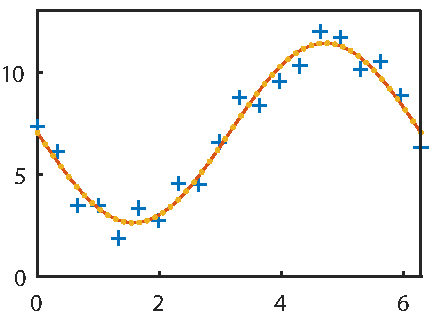
\includegraphics[width=8cm]{./figures/CurFit1.pdf}
\caption{运行结果} \label{CurFit_fig1}
\end{figure}

\Code{curveFit}

运行结果如\autoref{CurFit_fig1} 所示, 可见两种方法拟合出的曲线一致(红色的曲线和黄色的点线). 注意第 13 行使用了“Nelder-Mead 算法\upref{NelMea}” 中的函数 \x{NelderMead} 求函数句柄 \x{f} 的最小值.